\section{Introducción}
La mayoría de los modelos de aprendizaje de máquina tienen una arquitectura simple de dos capas. Sin embargo, al analizar el cerebro humano, se puede ver que este tiene muchos niveles de procesamiento. Se cree que cada capa aprende características o representaciones con niveles crecientes de abstracción. Por ejemplo, el modelo estándar del córtex humano sugiere que el cerebro primero extrae bordes, después pequeñas áreas, después superficies, después objetos, etc. Esta observación ha inspirado a un área del aprendizaje de máquina conocida como aprendizaje profundo que intenta replicar este tipo de arquitectura en una computadora.
\cite{Murphy:2012:MLP:2380985}

\vspace{1em}

El cerebro humano funciona de una manera diferente a una computadora normal. El cerebro es altamente complejo, no-lineal y funciona en paralelo. También tiene la capacidad de organizar sus componentes estructurales, conocidos como neuronas, para realizar tareas tales como reconocimiento de patrones a una velocidad muchas veces más rápida que la computadora más rápida que existe hoy en día.
\cite{Haykin:1998:NNC:521706}

\vspace{1em}

¿Cómo es capaz el cerebro humano de realizar dichas funciones? Desde el nacimiento, el cerebro ya tiene suficiente estructura y la habilidad para construir sus propias reglas de comportamiento a través de lo que conocemos como $``$experiencia$"$. El continuo desarrollo del sistema nervioso es posible gracias a la plasticidad del cerebro. La plasticidad permite al sistema nervioso de adaptarse al medio ambiente que lo rodea. Así como la plasticidad es esencial para el cerebro humano, también lo es con redes neuronales que están hechas de neuronas artificiales.
\cite{Haykin:1998:NNC:521706}

\vspace{1em}

Las redes neuronales artificiales se parecen al cerebro humano principalmente en dos aspectos: \\
1.- La red adquiere conocimiento de su ambiente a través de un proceso de aprendizaje.\\
2.- La fuerza de conexión entre las neuronas, conocido como los pesos sinápticos, se usa para almacenar el conocimiento adquirido. \\
El procedimiento que se usa para el proceso de aprendizaje se conoce como algoritmo de aprendizaje y su función es modificar los pesos sinápticos para mejorar el desempeño en la tarea que se quiere realizar. \cite{Haykin:1998:NNC:521706}

\vspace{1em}

Actualmente, el aprendizaje profundo sigue en desarrollo. Sin embargo, este ya resuelve una gran cantidad de tareas y es usado en la industria de manera importante. La mayoría de las tareas que consisten en mapear un vector de entrada a un vector de salida, y que son fáciles para una persona de realizar pueden ser resueltas con aprendizaje profundo si se tienen bases de datos y modelos suficientemente grandes. Otras tareas que no se pueden describir como mapear un vector a otro o que son suficientemente difíciles para que una persona tuviera que reflexionar para resolverlas, se mantienen fuera del alcance del aprendizaje profundo por ahora.
\cite{goodfellow-et-al-2016}

\vspace{1em}

En el siguiente capítulo se describirá el modelo básico de redes neuronales. Después, se explicarán conceptos importantes de regularización y de optimización. Finalmente, se explicarán los conceptos de redes neuronales recurrentes que se utilizarán para los experimentos de los capítulos 4 y 5.

\section{Redes neuronales prealimentadas}
Las redes neuronales prealimentadas, también conocidas como perceptrones multicapa son el modelo básico del aprendizaje profundo. El objetivo de estas es aproximar una función $f^*$. Una red neuronal prealimentada define un mapeo $y = f(x;\theta)$ y aprende el valor de los parámetros $\theta$ que resulten en la mejor función de aproximación. 

\vspace{1em}

Estos modelos se conocen como prealimentados porque la información fluye primero a través de la función al ser evaluada en $x$, después, a través de los cálculos intermedios utilizados para definir a $f$, y, finalmente, para obtener los datos de salida $y$. No hay conexiones cíclicas en las que un dato de salida del modelo sirva de nuevo como dato de entrada. Cuando esto sucede, el modelo se conoce como red neuronal recurrente.
\cite{goodfellow-et-al-2016}

\vspace{1em}

Las redes neuronales prealimentadas son redes porque se construyen componiendo varias funciones. Por ejemplo, se puede tener tres funciones $f^{(1)}$, $f^{(2)}$ y $f^{(3)}$ conectadas en una cadena para formar $f(x) = f^{(3)}(f^{(2)}(f^{(1)}(x)))$.

\vspace{1em}

La longitud de la red da la profundidad del modelo. Es esta terminología la que le da el nombre de aprendizaje profundo. La última capa se conoce como capa de salida. Los ejemplos de entrenamiento especifican directamente lo que la capa de salida debe hacer en cada punto $x$, esto es, debe producir un valor que sea cercano a $y$. El comportamiento de las otras capas no está especificado por los datos de entrenamiento, por lo que estas capas se conocen como capas ocultas. El algoritmo de aprendizaje usado es el que tiene que decidir cómo usar estas capas para implementar una aproximación de $f^*$.

\vspace{1em}

Finalmente, estas redes se conocen como neuronales porque están inspiradas en el cerebro. Cada capa es un vector y la dimensión de las capas ocultas determina el ancho del modelo. Cada elemento del vector puede pensarse que es una neurona, entonces, en vez de pensar a cada capa como una función de vector a vector, la podemos pensar como varias unidades que actúan en paralelo. Cada unidad se parece a una neurona en el sentido de que recibe datos de entrada de las otras unidades y calcula su valor de activación. La idea de usar muchas capas también proviene de la neurociencia. Sin embargo, la investigación actual en redes neuronales está guiada por muchos principios de matemáticas y de ingeniería y su objetivo no es modelar perfectamente al cerebro sino lograr generalización estadística.
\cite{goodfellow-et-al-2016}

\vspace{1em}

Para hacer la idea de una red neuronal más concreta, se dará un pequeño ejemplo con una capa oculta y dos unidades ocultas. Se quiere escoger la forma de nuestro modelo $f(x;\theta) = f^{(2)}(f^{(1)}(x))$. Las unidades ocultas $h$ de esta red neuronal son calculadas por una función $f^{(1)}(x;W,c)$. Los valores de estas unidades ocultas después son utilizados como datos de entrada para la segunda capa. 

\vspace{1em}

La segunda capa es la capa de salida del modelo y en este caso será una regresión lineal aplicada a $h$, es decir, $f^{(2)}(h;w,b) = w^Th + b$. Ahora bien, si $f^{(1)}$ fuera lineal, entonces $f$ sería lineal y eso no es lo que se busca. Por lo tanto, $f^{(1)}$, la función que describe los rasgos, tendrá que ser no lineal. La mayoría de las redes neuronales utilizan una transformación afín seguido de una función no-lineal llamada función de activación. 
\cite{goodfellow-et-al-2016}

\vspace{1em}

Si se hace esto, entonces $h=g(W^Tx+c)$ donde $W$ son los pesos de la transformación lineal y $c$ son los sesgos. La función de activación $g$ generalmente se aplica elemento a elemento, de tal forma que $h_i = g(x^TW_{:,i}+c_i)$. En la actualidad, la función de activación que se recomienda por default es la unidad lineal rectificada o ReLU por sus siglas en inglés (Rectified Linear Unit), definida por la función de activación $g(z) = max\{0,z\}$. \cite{conf/icml/NairH10}
\cite{goodfellow-et-al-2016}

Por lo tanto, el modelo definido es el siguiente:

\begin{equation}
\begin{split}
$$f(x;W,c,w,b) = w^Tmax\{0,W^Tx+c\}+b $$
\end{split}
\end{equation}

\subsection{Aprendizaje con descenso de gradiente}
Diseñar y entrenar una red neuronal no es muy diferente que entrenar cualquier otro modelo de aprendizaje de máquina con descenso de gradiente. La diferencia más grande entre los modelos lineales y las redes neuronales es que la no linealidad de las redes neuronales hace que muchas veces la función de pérdida se vuelva no convexa. Esto quiere decir que las redes neuronales generalmente se entrenan utilizando métodos de optimización iterativos basados en el descenso del gradiente. 
\cite{goodfellow-et-al-2016}

\subsubsection{Funciones de pérdida}
Un aspecto importante del diseño de una red neuronal es la elección de la función de pérdida. Afortunadamente, las funciones de costo para redes neuronales son muy parecidas a las de otros modelos paramétricos, como los modelos lineales.

\vspace{1em}
En la mayoría de los casos, el modelo paramétrico define una distribución $p(y|x;\theta)$ y se usa el principio de máxima verosimilitud. Esto quiere decir que la función de costo se calcula como la entropía cruzada entre los datos de entrenamiento y las predicciones del modelo. La función total de costo usada para entrenar una red neuronal generalmente combinará una de las funciones de pérdida vistas aquí con un término de regularización. \cite{goodfellow-et-al-2016}

\subsubsection{Unidades de salida}
La elección de la función de costo está altamente relacionada con la elección de la unidad de salida. La mayoría de las veces, simplemente se usa la entropía cruzada entre la distribución de los datos y la distribución del modelo. Por lo tanto, la elección de las unidades de salida determina la forma que tendrá la función de la entropía cruzada. 
\cite{goodfellow-et-al-2016}

\vspace{1em}

Una de las unidades de salida más utilizada es la función softmax. Esta usa cuando se quiere representar una distribución de probabilidades sobre una variable discreta con $n$ clases diferentes. Por lo tanto, se necesita producir un vector $\hat{y}$, con $\hat{y}_i = P(y=i|x)$. Se requiere no solo que cada elemento de $\hat{y}$ esté entre 0 y 1, pero también que el vector sume a 1 para que represente una distribución de probabilidad válida. 

\vspace{1em}

Para conseguir eso, primero una capa lineal predice las log probabilidades no normalizadas.


\begin{equation}
\begin{split}
$$z = W^T h + b$$
\end{split}
\end{equation}

Después, la función softmax puede exponenciar y normalizar $z$ para obtener el deseado $\hat{y}$. Por lo tanto, la función softmax está dada por:

\begin{equation}
\begin{split}
$$\mathrm{softmax}(z_i) = \frac{exp(z_i)}{\sum_j exp(z_j)}$$
\end{split}
\end{equation}

\subsubsubsection{Redes de densidad mixta}
Las redes de densidad mixta son redes neuronales que utilizan otro tipo de unidad de salida: la mezcla de gaussianas. Estos modelos son muy efectivos para modelar movimientos de objetos físicos como se hará en el capítulo 5 al describir movimientos de caligrafía. En la ecuación 3.2.4, se define una mezcla de gaussianas con $n$ componentes como una distribución de probabilidades condicionales.
\cite{goodfellow-et-al-2016}

\begin{equation}
\begin{split}
$$p(y|x) = \sum_{i=1}^n p(c=i|x) \mathcal{N}\left(y;\mu^{(i)}(x), \Sigma^{(i)}(x)\right)$$
\end{split}
\end{equation}

La red neuronal debe entregar tres datos de salida: un vector que defina a $p(c=i|x)$, una matriz que entregue $\mu^{(i)}(x)$ para toda $i$, y un tensor que entregue $\Sigma^{(i)}(x)$. Por un lado, el vector $p(c=i|x)$, donde $c$ es una variable latente, generalmente se obtiene de aplicar una función softmax a un vector de $n$ componentes. Por otro lado, las medias $\mu^{(i)}(x)$ indican el centro de la $i$-ésima componente gaussiana, por lo que si $y$ es un vector de $d$ dimensiones, la red nos debe de entregar una matriz de $n\times d$ que contenga a los $n$ vectores de dimensión $d$. Finalmente, $\Sigma^{(i)}(x)$ calculará la matriz de covarianza para cada componente $i$.
\cite{goodfellow-et-al-2016}

\subsection{Unidades ocultas}
Las unidades ocultas es un tema exclusivo de las redes neuronales, puesto que estas no aparecen en los algoritmos convencionales de aprendizaje de máquina. El diseño de las unidades ocultas es un tema de investigación muy activo y no existen todavía principios teóricos definitivos que guíen el tema.\cite{goodfellow-et-al-2016}

\vspace{1em}

 Existen varias unidades ocultas, incluyendo la ReLU, que no son diferenciables en todos sus puntos. Se podría pensar que esto invalida a las funciones para ser utilizadas con algoritmos de descenso de gradiente. Pero en la práctica, descenso de gradiente funciona suficientemente bien. Esto es en parte porque los algoritmos con redes neuronales generalmente no llegan a un mínimo local de la función objetivo, sino que simplemente reducen su valor significativamente. \cite{goodfellow-et-al-2016}

\subsection{Diseño de la arquitectura de la red}
Otra consideración importante para el diseño de la red es su arquitectura, es decir, su estructura en términos generales: cuántas unidades tendrá y cómo se conectan estas unidades entre ellas. La mayoría de las redes neuronales están organizadas en capas y estas capas se conectan en cadena, donde cada capa es una función de la capa que le precede. Con esta estructura, la primera capa está dada por:
\cite{goodfellow-et-al-2016}


\begin{equation}
\begin{split}
$$h^{(1)} = g^{(1)}(W^{(1)^T}x+b^{(1)}), $$
\end{split}
\end{equation}

la segunda capa por:

\begin{equation}
\begin{split}
$$h^{(2)} = g^{(2)}(W^{(2)^T}h^{(1)}+b^{(2)}), $$
\end{split}
\end{equation}

y así sucesivamente donde $x$ son los datos de entrada, $W$ las matrices de pesos, $b$ el vector de sesgo y $g$ las funciones de activación. Con este tipo de arquitectura, las principales consideraciones que se tienen que hacer son la profundidad y el ancho del modelo. La arquitectura ideal para cierta tarea debe ser encontrada mediante la experimentación y monitoreando el error de validación.
\cite{goodfellow-et-al-2016}

\subsection{Propagación hacia atrás}
En las redes neuronales prealimentadas, cuando le damos al modelo datos de entrada $x$ para producir un dato de salida $\hat{y}$, la información fluye hacia adelante a través de la red. Los datos de entrada $x$ proveen la información necesaria que luego se propaga en las unidades ocultas de cada capa para finalmente producir $\hat{y}$. Esto es llamado propagación hacia adelante. Durante el entrenamiento, la propagación hacia adelante continúa hasta producir un costo escalar $J(\theta)$. El algoritmo de propagación hacia atrás permite a la información de fluir hacia atrás a través de la red para calcular el gradiente.
\cite{goodfellow-et-al-2016}
\cite{Rumelhart:1986:LIR:104279.104293}

\vspace{1em}

A menudo se piensa que el algoritmo de propagación hacia atrás es todo el algoritmo de aprendizaje para redes neuronales. Esto es falso, el algoritmo de propagación hacia atrás solo se refiere al método para calcular el gradiente, mientras que otro algoritmo, descenso de gradiente estocástico, es usado para aprender utilizando este gradiente. 
\cite{goodfellow-et-al-2016}

\subsection{Propagación hacia atrás con gráficas computacionales}
Para describir con más formalidad el algoritmo de propagación hacia atrás, se utilizará un lenguaje de gráficas computacionales. Cada nodo de la gráfica indicará una variable. También se definirá una operación como una función de una o más variables cuyo valor de salida es otra variable. Si la variable $y$ se calcula aplicando una operación a la variable $x$, entonces se trazará una arista dirigida de $x$ a $y$.

\vspace{1em}

Ahora bien, al realizar el algoritmo de propagación hacia atrás, se utilizará la gráfica computacional para decidir el orden de las operaciones y aplicar la regla de la cadena para calcular el gradiente. La regla de la cadena generalizada dice lo siguiente: sea $x \in \mathbb{R}^n$, $y \in \mathbb{R}^m$, $g$ es una función de $\mathbb{R}^m$ a $\mathbb{R}^n$, $f$ es una función de $\mathbb{R}^n$ a $\mathbb{R}$. Si $y = g(x)$, $z = f(y)$, entonces:
\begin{equation}
\begin{split}
$$\frac{\partial z}{\partial x_i}=\sum_j \frac{\partial z}{\partial y_j}\frac{\partial y_j}{\partial x_i}$$
\end{split}
\end{equation}

En notación vectorial, esto es equivalente a:
\begin{equation}
\begin{split}
$$\nabla_x z = \left(\frac{\partial y}{\partial x}\right)^T \nabla_y z$$,
\end{split}
\end{equation}

donde $\frac{\partial y}{\partial x}$ es la matriz jacobiana de $g$ con dimensiones de $n \times m$.
De aquí se puede ver que el gradiente de una variable $x$ se puede obtener al multiplicar la matriz jacobiana $\frac{\partial y}{\partial x}$ por el gradiente $\nabla_y z$. El algoritmo de propagación hacia atrás consiste en realizar este producto para cada operación en la gráfica.
\cite{goodfellow-et-al-2016}

\section{Regularización en aprendizaje profundo}
En la subsección 2.3.2 se dio una breve introducción a lo que es regularización. Regularización se refiere a cualquier modificación que se hace a un algoritmo de aprendizaje para reducir su error de generalización, pero no su error de entrenamiento. En esta sección, se analizarán algunos de los métodos de regularización que funcionan mejor en aprendizaje profundo. \cite{goodfellow-et-al-2016}

\vspace{1em}

Vincent Vanhoucke, investigador de Google, utiliza una metáfora para dar una mejor idea de cómo funciona regularización en su curso de aprendizaje profundo. Vanhoucke explica que hay un problema general al hacer optimización numérica que él conoce como el problema de los pantalones $``$skinny$"$. Este tipo de pantalones se ven muy bien y se ajustan perfectamente, pero es muy difícil de entrar en ellos, por lo que la mayoría de las personas acaban usando pantalones que les quedan un poco grandes. Lo mismo pasa con las redes profundas: una red que tenga el tamaño justo para los datos es muy difícil de optimizar, por lo que en la práctica se utilizan redes que son muy grandes para los datos y después se intenta que no sobreajusten. A continuación, se describirá el método de detención temprana y el método de $``$dropout$"$.
\cite{deeplearningbygoogle}

\subsection{Detención temprana}
La técnica de detención temprana se basa en una idea muy simple: utilizar los parámetros que minimizan el error de validación. En general, al utilizar modelos grandes que puedan sobrestimar a los datos, sucede que el error de entrenamiento disminuye a través del tiempo, pero el error de validación comienza a aumentar. Por lo tanto, se obtiene un mejor error de validación y probablemente de prueba al utilizar los parámetros que entregaron el menor error de validación.
\cite{goodfellow-et-al-2016}

\vspace{1em}

Por lo tanto, lo que se hace en la práctica es guardar los parámetros del modelo cada vez que el error de validación mejore. Al finalizar el algoritmo, se entregarán los parámetros guardados en vez de los últimos parámetros. El algoritmo terminará si los parámetros no han mejorado al error de validación en un número preespecificado de iteraciones. Este es el tipo más común de regularización en aprendizaje profundo por su efectividad y simplicidad.
\cite{goodfellow-et-al-2016}

\subsection{Dropout}
Dropout es otro método de regularización que emergió recientemente (Srivastana et al., 2014) y funciona muy bien debido a su bajo costo computacional. Básicamente, dropout funciona de la siguiente manera. Si se tienen dos capas que se conectan entre sí, los valores que van de una capa a otra se conocen como activaciones. Lo que hace dropout es que cada una de estas activaciones se hace 0 con una probabilidad $p$, donde generalmente $p=0.5$ para las capas ocultas. En otras palabras, lo que está haciendo dropout es $``$destruir$"$ la mitad de los datos.
\cite{goodfellow-et-al-2016}
\cite{Srivastava:2014:DSW:2627435.2670313}
\cite{deeplearningbygoogle}

\vspace{1em}

Esta idea puede sonar un poco rara, pero Vincent Vanhoucke explica la intuición detrás del éxito del método en su curso de aprendizaje profundo: la red no puede confiar en ninguna activación porque podría ser convertida en cero en cualquier momento, por lo que la red aprende una representación redundante para estar segura que al menos alguna parte de la información permanezca. En la práctica, esto hace a la red más robusta y previene sobreajustar a los datos. 
\cite{goodfellow-et-al-2016}
\cite{deeplearningbygoogle}

%\section{Regularization for deep learning}
%\subsection{Parameter norm penalties}
%\subsection{Norm penalties as constrained optimization}
%\subsection{Dataset augmentation}
%\subsection{Noise robustness}
%\subsection{Dropout}


\section{Optimización en aprendizaje profundo}
La optimización es uno de los aspectos más importantes a considerar al hablar de aprendizaje profundo. La optimización de la redes neuronales, es decir, encontrar los parámetros $\theta$ que minimizan la función de pérdida $J(\theta)$, es un problema bastante complicado. Es por esto que se han creado técnicas especiales para resolver este desafío. En la sección 2.5, se explicó el algoritmo básico de aprendizaje de máquina, gradiente estocástico, por lo que esta sección se dedicará a describir algunos de los algoritmos más avanzados que se usarán en los capítulos 4 y 5.

\vspace{1em}

El aprendizaje de máquina tiene diferencias considerables con la optimización pura. En el aprendizaje de máquina se aprende indirectamente, es decir, normalmente se busca mejorar una medida de desempeño $P$, pero, por la dificultad de medir a $P$, se utiliza una función de pérdida diferente $J(\theta)$ con la esperanza de mejorar $P$. En cambio, en la optimización pura, minimizar a $J(\theta)$ es un objetivo en sí mismo.
\cite{goodfellow-et-al-2016}

\subsection{Momentum}
El método del gradiente estocástico que se estudió en la sección 2.5 es uno de los algoritmos claves de optimización en redes neuronales. Sin embargo, este método puede ser un poco lento. El método de momentum está diseñado para acelerar el aprendizaje al acumular un promedio de gradientes con decaimiento exponencial. Este método introduce una variable $v$ que tiene el rol de la velocidad debido a que es la dirección y velocidad a la que los parámetros se mueven por el espacio de parámetros. Un hiperparámetro $\alpha$ determina qué tan rápido las contribuciones de gradientes previos decaen exponencialmente. La regla de actualización es la siguiente:
\cite{goodfellow-et-al-2016}

\begin{equation}
\begin{split}
$$v \leftarrow \alpha v - \epsilon \nabla_{\theta} \left(\frac{1}{m}\sum_{1}^{m} L(x^{(i)},y^{(i)},\theta\right)$$
\end{split}
\end{equation}

\begin{equation}
\begin{split}
$$\theta \leftarrow \theta + v$$
\end{split}
\end{equation}

\subsection{Algoritmos con tasas de aprendizaje adaptativas}
Elegir la tasa de aprendizaje es muy importante al optimizar redes neuronales debido a que esta elección tiene un impacto significativo en el desempeño del modelo. El algoritmo de momentum que se vio en la subsección anterior puede mitigar estos problemas hasta cierto punto, pero lo hace a expensas de tener que introducir un nuevo hiperparámetro. Para resolver este problema se han creado algoritmos que utilizan una tasa de aprendizaje diferente para cada parámetro y automáticamente adaptan estas tasas a lo largo del entrenamiento. Algunos los algoritmos con tasas de aprendizaje adaptativas más conocidos son los siguientes: AdaGrad, RMSProp y Adam.
\cite{goodfellow-et-al-2016}

%\section{Optimization for training deep models}
%\subsection{How learning differs from pure optimization}
%\subsection{Challenges in neural network optimization}
%\subsection{Basic algorithms}
%\subsubsection{SGD}
%\subsubsection{Momentum}
%\subsection{Parameter initialization strategies}
%\subsection{Algorithms with adaptative learning rates}
%\subsection{Aproximate second-order methods}

\section{Redes neuronales recurrentes}
Las redes neuronales recurrentes son una familia de redes neuronales utilizadas para procesar datos secuenciales. Estas redes permiten procesar sucesiones mucho más grandes de las que podría procesar una red neuronal convencional, además de poder procesar sucesiones con longitud variable.
\cite{goodfellow-et-al-2016}
\cite{Rumelhart:1986:LIR:104279.104293}

\vspace{1em}

Una de las claves que llevó a desarrollar las redes neuronales recurrentes es la idea de compartir parámetros a través de diferentes partes del modelo. Compartir parámetros hace posible extender y aplicar el modelo a sucesiones de diferentes longitudes y generalizar a través de ellas. Compartir parámetros es especialmente importante cuando un pedazo de información puede ocurrir en diferentes posiciones dentro de la sucesión. Por ejemplo, si se consideran los dos enunciados $``$En 2011, entré al ITAM$"$ y $``$Entré al ITAM en 2011$"$. Si se le pide a un modelo de aprendizaje de máquina leer los dos enunciados y extraer el año en el que el narrador entró al ITAM, debería reconocer 2011 como un pedazo clave de información sin importar si apareció en la quinta o en la tercera posición del enunciado. Una red neuronal convencional tendría parámetros separados para cada variable de entrada, por lo que tendría que aprender todas las reglas del lenguaje de manera separada para cada posición en el enunciado. En cambio, una red neuronal recurrente comparte los pesos a través de las diferentes ventanas de tiempo.
\cite{goodfellow-et-al-2016}

\subsection{Desdoblando gráficas computacionales}
Como se vio en la sección 3.2.5, las gráficas computacionales permiten formalizar la estructura de una red neuronal. En esta sección, se explicará cómo desdoblar una red neuronal recurrente hacia una gráfica computacional que tenga estructura repetitiva. Al desdoblar la gráfica, se obtendrá una gráfica que comparte parámetros a través de una red profunda. \cite{goodfellow-et-al-2016}

\vspace{1em}

Por ejemplo, si se considera la forma clásica de un sistema dinámico:
\begin{equation}
\begin{split}
$$s^{(t)}=f(s^{(t-1)};\theta),$$
\end{split}
\end{equation}
donde $s^{(t)}$ es el estado del sistema. La ecuación $(3.3.1)$ se considera recurrente debido a que la definición de $s$ en el tiempo $t$ alude a la misma definición, pero en el tiempo $t-1$. Para un número finito de pasos $\tau$, la gráfica puede ser desdoblada aplicando la definición $\tau-1$ veces. Por ejemplo, si se desdobla la ecuación que se definió $\tau=3$ pasos de tiempo, se obtiene:

\begin{equation}
\begin{split}
$$s^{(3)}=f(s^{(2)};\theta)=f(f(s^{(1)};\theta);\theta$$
\end{split}
\end{equation}

En otras palabras, si se desdobla la ecuación al aplicar la definición, se obtiene una expresión que no involucra recurrencia. Esta expresión se puede representar por una gráfica tradicional sin ciclos como se muestra en la figura 3.1.
\cite{goodfellow-et-al-2016}

\begin{figure}[!ht]
\begin{center}
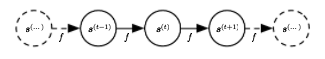
\includegraphics[width=150mm, scale = 0.8]{./imag/unfold.png}
\end{center}
\caption{Gráfica desdoblada de la ecuación 3.5.1. Cada nodo representa el estado en un tiempo $t$ y la función $f$ mapea el estado $t$ al estado $t+1$. Los mismos parámetros $\theta$ se utilizan para todos los pasos de tiempo. Figura tomada de (Goodfellow et al, 2016). }
\end{figure}

 
\vspace{1em}

Otro ejemplo sería considerar un sistema dinámico afectado por una señal externa $x^{(t)}$,

\begin{equation}
\begin{split}
$$h^{(t)}=f(h^{(t-1)},x^{(t)};\theta)$$
\end{split}
\end{equation}

Muchas redes neuronales recurrentes utilizan la ecuación 3.5.3 para definir su estado oculto o $``$hidden state$"$ en inglés; por eso, se utilizará la letra $h$ para describir la sucesión. Una red neuronal recurrente normalmente tiene también una capa de salida que lee información del estado $h$ para hacer predicciones.
\cite{goodfellow-et-al-2016}


\begin{figure}[h]
\begin{center}
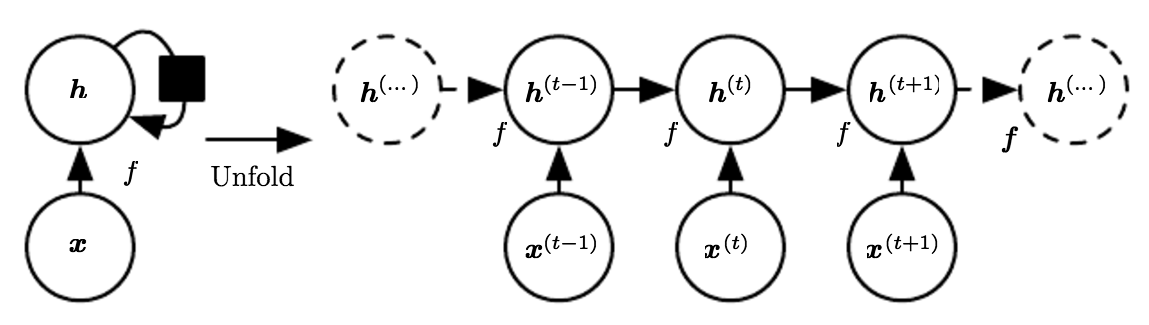
\includegraphics[width=150mm, scale = 0.8]{./imag/unfold2.png}
\end{center}
\caption{Red neuronal recurrente sin capa de salida. Esta red incorpora información de los datos de entrada $x$ al estado $h$ a través del tiempo. El cuadrado negro en las gráficas indica el retraso en un paso de tiempo. Figura tomada de (Goodfellow et al, 2016).}
\end{figure}

\subsection{Redes neuronales recurrentes}
Con los conceptos hasta ahora desarrollados, ya se pueden construir una variedad de redes neuronales. Se ejemplificará esto con el modelo básico que usará en los capítulos 4 y 5 para desarrollar los experimentos. Este modelo, mostrado en la figura 3.3, es una red neuronal que produce un dato de salida en cada paso de tiempo y tiene conexiones recurrentes entre las capas ocultas.
\cite{goodfellow-et-al-2016}
\cite{DBLP:journals/corr/Graves13}

\begin{figure}[h]
\begin{center}
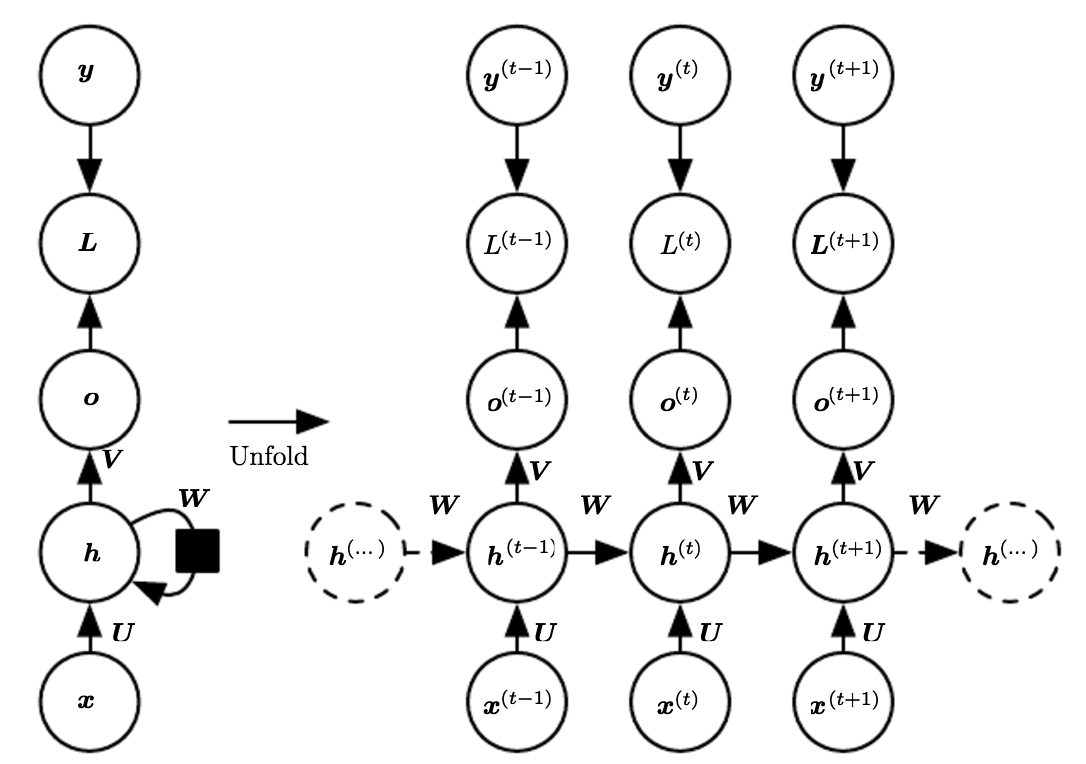
\includegraphics[width=150mm, scale = 0.8]{./imag/unfold3.png}
\end{center}
\caption{Una red neuronal recurrente enrollada y desenrollada. Con la sucesión de datos de entrada $x$, se calculan los datos de salida $o$ y con estos y las etiquetas $y$ se puede computar la función de pérdida correspondiente $L$. También se puede ver que $U$ es la matriz de pesos de los datos de entrada a las capas ocultas, $W$ es la matriz de pesos que conecta la recurrencia de las unidades ocultas y $V$ es la matriz de pesos de las unidades ocultas a los datos de salida $o$. Figura tomada de (Goodfellow et al, 2016).}
\end{figure}

\vspace{1em}

A continuación, se describirán las ecuaciones de propagación hacia adelante de este modelo. Se supondrá que los datos de salida son discretos, como se hará en el experimento 4, y que la función de activación es la función ReLU. Las siguientes son las ecuaciones para los pasos de tiempo $t=1$ a $t=\tau$.

\begin{equation}
\begin{split}
$$a^{(t)}=b+Wh^{(t-1)}+Ux^{(t)}$$
\end{split}
\end{equation}
\begin{equation}
\begin{split}
$$h^{(t)}=ReLU(a^{(t)})$$
\end{split}
\end{equation}
\begin{equation}
\begin{split}
$$o^{(t)}=c+Vh^{(t)}$$
\end{split}
\end{equation}
\begin{equation}
\begin{split}
$$\hat{y}^{(t)}=\mathrm{softmax}(o^{(t)})$$
\end{split}
\end{equation}

Si la función de pérdida, $L^{(t)}$, es log-verosimilitud negativa de $y^{(t)}$ dado $x^{(1)}, ...,x^{(t)}$, entonces 

\begin{equation}
\begin{split}
$$L(\{x^{(1)},...,x^{(\tau)}\},\{y^{(1)},...,y^{(\tau)}\})$$
\end{split}
\end{equation}
\begin{equation}
\begin{split}
$$=\sum_tL^{(t)}$$
\end{split}
\end{equation}
\begin{equation}
\begin{split}
$$=-\sum_t log p_{model}(y^{(t)}|\{x^{(1)},...,x^{(t)}\})$$
\end{split}
\end{equation}

donde $p_{model}(y^{(t)}|\{x^{(1)},...,x^{(t)}\})$ es la entrada de $\hat{y}^{(t)}$ que corresponde a la etiqueta $y^{(t)}$. Para calcular al gradiente se hace la propagación hacia adelante al moverse en la figura (3.3) de izquierda a derecha, y luego la propagación hacia atrás se hace de derecha a izquierda de esta gráfica computacional extendida. 
\cite{goodfellow-et-al-2016}

\subsection{Dependencias de largo plazo}
El problema de las dependencias de largo plazo aparece cuando la gráfica computacional es demasiado larga, lo cual sucede fácilmente al desdoblar la gráfica en las redes neuronales recurrentes. En este caso, como los mismos parámetros se propagan hacia atrás por muchos pasos, el algoritmo de propagación hacia atrás se vuelve inestable y se puede llegar al problema del gradiente evanescente o al problema del gradiente explosivo. Se explicará a continuación el porqué.
\cite{goodfellow-et-al-2016}
\cite{Haykin:1998:NNC:521706}

\vspace{1em}

Supongamos que una gráfica computacional contiene un camino que consiste en multiplicar repetidamente por una matriz $W$. Después de $t$ pasos, esto es equivalente a multiplicar por $W^t$ y si la descomposición en valores propios de $W$ es $W^t = Vdiag(\lambda)V^{-1}$, entonces:

\begin{equation}
\begin{split}
$$W^t = (Vdiag(\lambda)V^{-1})^t=Vdiag(\lambda)^tV^{-1}$$
\end{split}
\end{equation}

Por lo que los valores propios, $\lambda_i$ cuyo valor absoluto no sea cercano a $1$, se harán muy grandes si son mayores que uno, causando el problema del gradiente explosivo, o se reducirán rápidamente a cero, causando el problema del gradiente evanescente.
\cite{goodfellow-et-al-2016}
\cite{Haykin:1998:NNC:521706}

\vspace{1em}

Se explicará a continuación el método para resolver el problema del gradiente explosivo: recorte de gradiente. La solución para el problema del gradiente evanescente, la memoria corta de largo plazo, se explicará en la siguiente sección.

\subsection{Recorte de gradiente}
Una técnica para evitar el problema del gradiente explosivo es el recorte de gradiente. Este es un problema relevante, pues si el gradiente de un parámetro es demasiado grande, al hacer la actualización, se puede acabar muy lejos del punto original y en una región donde la función objetivo tenga un valor mayor. En la figura 3.4, tomada de (Goodfellow et al., 2016), se da un ejemplo de las complicaciones que pueden aparecer.
\cite{goodfellow-et-al-2016}
\cite{DBLP:journals/corr/abs-1211-5063}


\begin{figure}[h]
\begin{center}
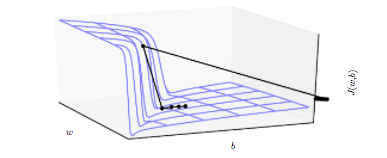
\includegraphics[width=150mm, scale = 0.8]{./imag/clipping.png}
\end{center}
\caption{La función de pérdida $J(w,b)$ puede contener puntos que tengan derivadas muy grandes. Si los parámetros están cerca de estos puntos, al avanzar con descenso de gradiente, se llegará a un punto muy lejano, lo cual podría afectar a la optimización.}
\end{figure}

\vspace{1em}

La solución a esto es recortar el gradiente. Es decir, elegir una cota máxima para las entradas del gradiente y, justo antes de hacer la actualización de parámetros, escalar al gradiente para que se respete la cota máxima.
\cite{goodfellow-et-al-2016}
\cite{DBLP:journals/corr/Graves13}
\cite{DBLP:journals/corr/abs-1211-5063}

\section{Memoria larga de corto plazo}
La memoria larga de corto plazo es un tipo de unidad recurrente con $``$compuertas$"$. Estas compuertas se construyen de tal forma que los caminos de la gráfica computacional tengan derivadas que no exploten ni se desvanezcan. De esta forma se puede acumular información por un largo periodo de tiempo, y si la información ha sido usada y el sistema no la necesita más, también la puede borrar de la memoria. En la figura 3.5, tomada de (Goodfellow et al., 2016), se muestra la estructura de una $``$celda$"$ de memoria larga de corto plazo. Nos referiremos a estas como LSTM de ahora en adelante, por su nombre en inglés $``$long short-term memory$''$.
\cite{Gers:2000}
\cite{goodfellow-et-al-2016}
\cite{Hochreiter:1997:LSM:1246443.1246450}

\vspace{1em}

\begin{figure}[h]
\begin{center}
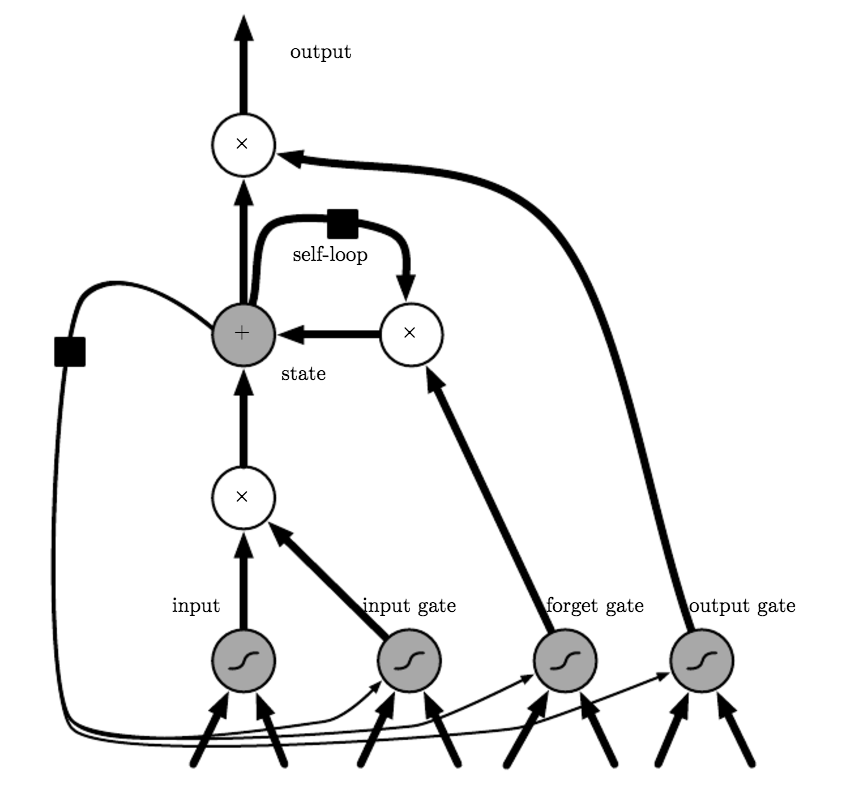
\includegraphics[width=150mm, scale = 0.8]{./imag/lstm.png}
\end{center}
\caption{Diagrama de la celda LSTM de la red neuronal. Estas celdas están conectadas recurrentemente entre ellas, remplazando las unidades ocultas de las redes recurrentes tradicionales. Los datos de entrada pasan por una red neuronal tradicional. Después este valor puede ser acumulado en el estado de la celda si la compuerta de entrada sigmoidal lo permite. La unidad que contiene al estado de la celda tiene un estado recurrente a sí misma, cuyo peso es controlado por la compuerta de olvido. Las datos de salida de la celda pueden ser $``$apagados$"$ por la compuerta de salida. Todas las unidades de compuerta tienen una función de activación no lineal y usualmente sigmoidal. Figura tomada de (Goodfellow et al. 2016). }
\end{figure}

\vspace{1em}

A continuación se presentarán las ecuaciones de propagación hacia adelante para la red neuronal recurrente LSTM con una capa oculta. El componente principal de una celda LSTM es el estado de la celda $s_i^{(t)}$, el cual tiene una conexión recurrente a sí mismo que es controlado por la compuerta de olvido $f_i^{(t)}$ cuyo valor se modula entre 0 y 1 por una unidad sigmoidal. Por lo tanto si $x^{(t)}$ es el vector de datos de entrada actual, $h^{(t)}$ es el vector de la capa oculta actual que contiene los datos de salida de las celdas LSTM, y $b^f$, $U^f$ y $W^f$ son los sesgos, pesos de entrada y pesos recurrentes para la compuerta de olvido respectivamente, entonces:
\cite{goodfellow-et-al-2016}
\cite{DBLP:journals/corr/Graves13}
\cite{DBLP:journals/corr/SakSB14}

\begin{equation}
\begin{split}
$$f_i^{(t)}=\sigma\left(b_i^f+\sum_j U_{i,j}^fx_j^{(t)}+\sum_j W_{i,j}^f h_j^{(t-1)}\right)$$
\end{split}
\end{equation}

Ahora bien, la compuerta de entrada exterior $g_i^{(t)}$ se calcula de manera similar a la compuerta de olvido pero con sus propios parámetros:

\begin{equation}
\begin{split}
$$g_i^{(t)} = \sigma \left(b_i^g+\sum_j U_{i,j}^g x_j^{(t)}+ \sum_j W_{i,j}^g h_j^{t-1}\right)$$
\end{split}
\end{equation}

Por lo tanto si $b$, $U$ y $W$ son los sesgos, pesos de entrada y pesos recurrentes de la celda LSTM, entonces el estado $s_i^{(t)}$ se actualiza de la siguiente manera:

\begin{equation}
\begin{split}
$$s_i^{(t)}=f_i^{(t)}s_i^{(t-1)}+g_i^{(t)} tanh\left(b_i+\sum_j U_{i,j}x_j^{(t)}+ \sum_j W_{i,j}^g h_j^{(t-1)} \right)$$
\end{split}
\end{equation}

Para calcular el vector de salida de la celda LSTM, $h_i^{(t)}$, se utiliza una compuerta de salida $q_i^{(t)}$ de manera similar a como se hizo con el estado de la celda:
\cite{goodfellow-et-al-2016}
\cite{DBLP:journals/corr/Graves13}
\cite{DBLP:journals/corr/SakSB14}

\begin{equation}
\begin{split}
$$q_i^{(t)}=\sigma\left(b_i^o+\sum_j U_{i,j}^o x_j^{(t)}+\sum_j W_{i,j}^o h_j^{t-1}\right)$$
\end{split}
\end{equation}

\begin{equation}
\begin{split}
$$h_i^{(t)}=tanh\left(s_i^{(t)}\right)q_i^{(t)}$$
\end{split}
\end{equation}

Se ha mostrado que las redes neuronales recurrentes que utilizan celdas LSTM pueden aprender y modelar sucesiones complejas con estructura de largo alcance. A continuación, en los capítulos 4 y 5, se modelarán este tipo de sucesiones utilizando estos modelos.
\cite{goodfellow-et-al-2016}
\cite{DBLP:journals/corr/Graves13}
\cite{DBLP:journals/corr/SakSB14}
\cite{DBLP:journals/corr/SutskeverVL14}







